\newpage
\section*{Pruebas unitarias}
\subsection*{Smart Owl}
\begin{center}
  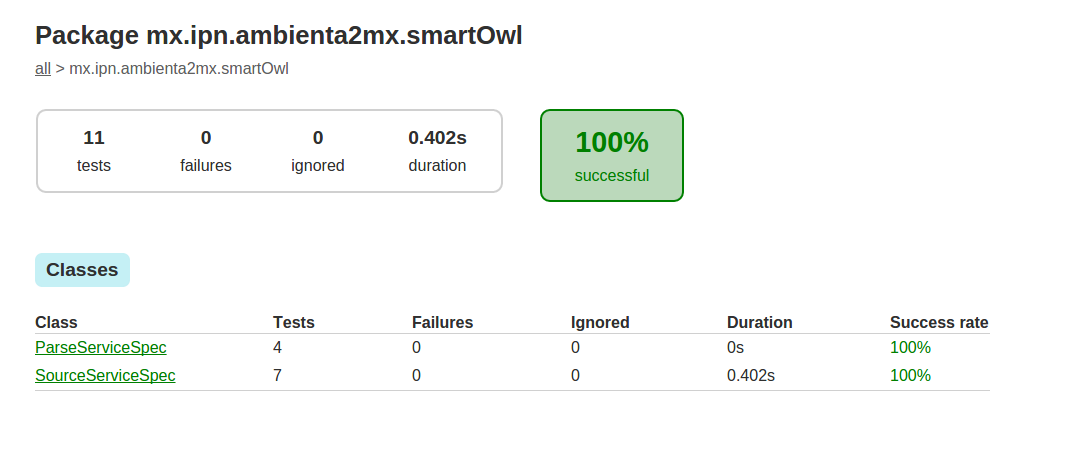
\includegraphics[width=\textwidth]{images/SmartOwlTest1}
\end{center}

\begin{center}
  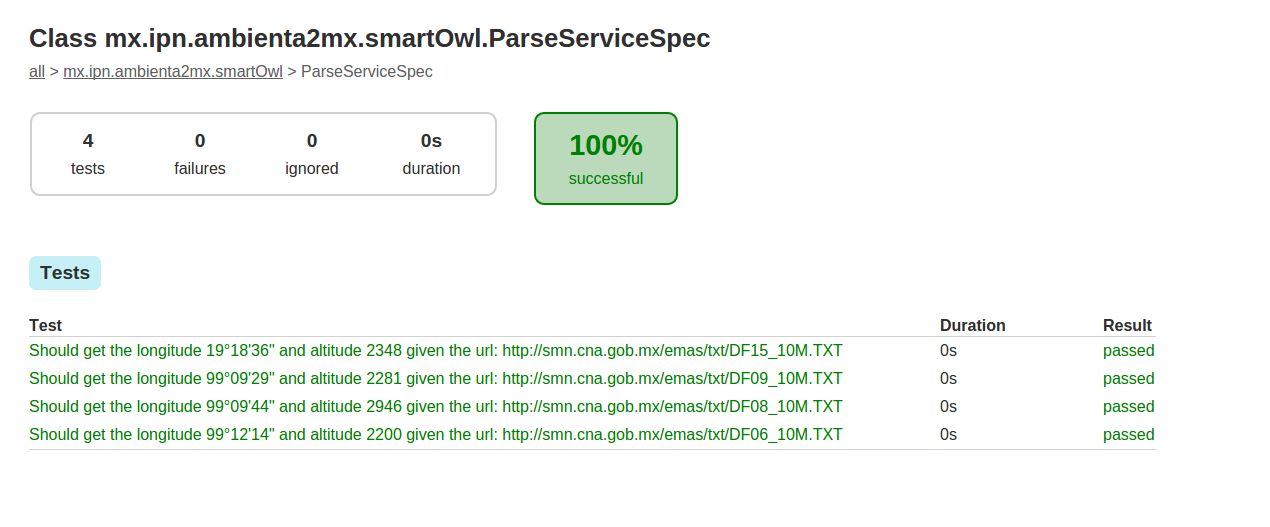
\includegraphics[width=\textwidth]{images/SmartOwlTest2}
\end{center}

\begin{center}
  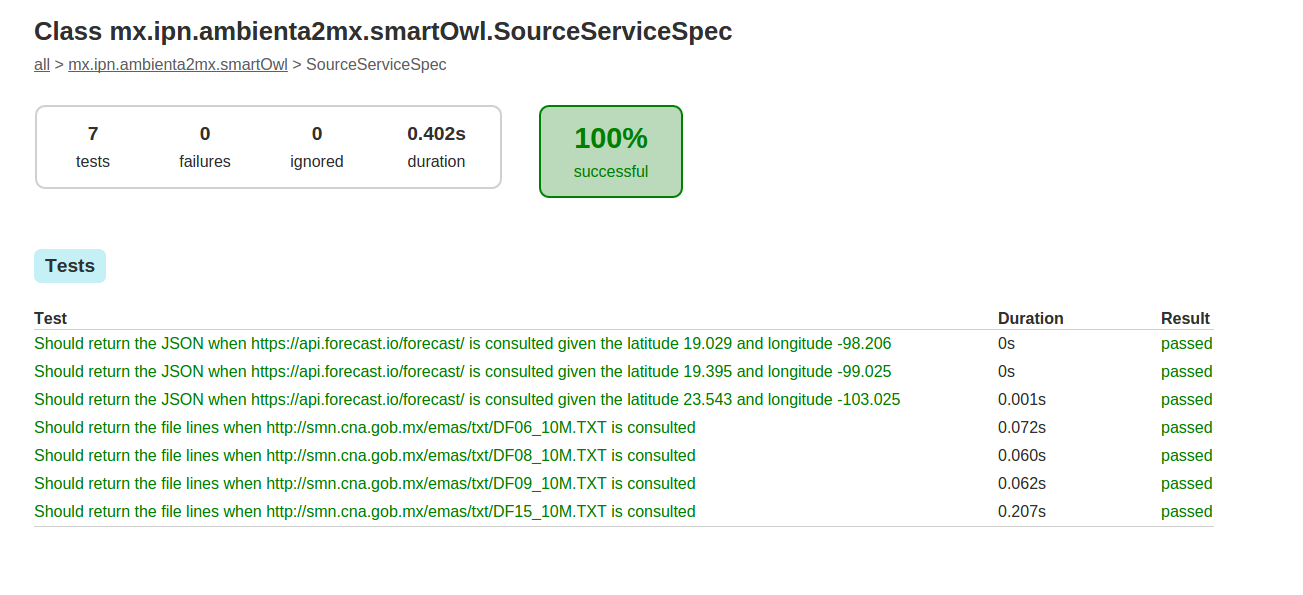
\includegraphics[width=\textwidth]{images/SmartOwlTest3}
\end{center}
\addcontentsline{toc}{chapter}{Anexo 1: Pruebas Unitarias}
%
% User stories
%
\newpage
\section*{Historias de Usuario}
\subsection*{SmartOwl}
\begin{itemize}
  \item US1 Estándarizar información de diferentes fuentes
  \begin{itemize}
    \item \textbf{Como} usuario de SmartOwl
    \item \textbf{Quiero} consultar la información climática actual
    \item \textbf{De tal manera} que la información se obtenga con un estándar definido
  \end{itemize}
  \item Criterios de Aceptación
  \begin{itemize}
    \item Mostrar de qué región del país provienen los valores de las variables.
    \item La información debe presentarse en formato JSON, XML y texto plano dependiendo del parámetro contentType que se envíe en la petición.
  \end{itemize}
\end{itemize}

\subsection*{Friendly Dolphin}
  \begin{itemize}
    \item US1 Reporte de información climática actual
    \begin{itemize}
      \item \textbf{Como} usuario de Friendly Dolphin
      \item \textbf{Quiero} consultar la información climática actual
      \item \textbf{De tal manera} que pueda generar un reporte con la información estandarizada.
    \end{itemize}
    \item Criterios de Aceptación
    \begin{itemize}
      \item Seleccionar una región del pais.
      \item Se deberá mostrar la información en texto plano.
      \item Opción para exportar la información en formato JSON o XML.
    \end{itemize}
  \end{itemize}
  \begin{itemize}
    \item US2 Historial de información climática
    \begin{itemize}
      \item \textbf{Como} usuario de Friendly Dolphin
      \item \textbf{Quiero} consultar el historial de los datos climáticos.
      \item \textbf{De tal manera} que pueda visualizar de manera gráfica el cambio de los valores de las variables climáticas a través de un periodo de tiempo
    \end{itemize}
    \item Criterios de Aceptación
    \begin{itemize}
      \item Consultar la información entre una fecha de Inicio y una fecha Final.
      \item Se deberá mostrar la información de las variables climáticas en el periodo seleccionado.
      \item Opción para exportar la información en formato JSON o XML.
    \end{itemize}
  \end{itemize}
\addcontentsline{toc}{chapter}{Anexo 2: Historias de Usuario.}
%
% RESTful Services
%
\newpage
\section*{Servicios REST}
\paragraph{La ventaja al usar servicios de tipo REST, es la sencillez al cambiar el contenido que se expone sin tener que cambiar o generar un protocolo de comunicación ya que toma como base HTTP}.
\paragraph{Simplemente es necesario con un cliente, desde un navegador web hasta clientes dedicados a servicios REST, para poder accedera a los recursos expuestos. Todas las API's rest siguen una convención de verbos tomados de la base de HTTP (GET, POST, PUT, DELETE).}
\paragraph{En comparación con servicios de tipo SOAP, no se requiere una alta atomicidad y ni transacciones, una de las razones por la que los servicios WS suelen ser usados.}
\paragraph{Finalmente, los servicios de tipo REST pueden tener respuestas en diversos formatos, principalmente JSON y XML, esto brinda al desarollador o a la persona que consula como tratar la respuesta por bibliotecas de terceros o nativas.}
\paragraph{El soporte para formatos JSON es nativo en los navegadores web, otra de las razones por las cuales éstos servicios han ido ganando mercado ya que el desarrollo de aplicaciones Web ha aumentado de forma drástica en los últimos años. \cite{31}}
\addcontentsline{toc}{chapter}{Anexo 3: Servicios REST}

%
% External sources
%

\newpage
\section*{Fuentes externas de datos}
\paragraph{Una de las fuentes usadas fue la de \textbf{CONAGUA}, institución de caracter público y mantenida por el Gobierno Federal, cuya misión es preservar las aguas nacionales y bienes públicos para su administración sustentable.}
\paragraph{Una de las funciones de la CONAGUA es contar con los registros de clima e información ambiental de las fuentes que tiene distribuidas a lo largo del territorio nacional, éstas fuentes carecen de un formato definido lo cual complica en gran forma el análisis de datos.\cite{32}}
\paragraph{Para el desarrollo de la etapa final del proyecto se procedió a realizar un scrapping de la información expuesta por sus servicios y adaptarlos al modelo de datos propuesto por el equipo de trabajo.}
\paragraph{A continuación se muestra un ejemplo de la información brindada por los servicios de la CONAGUA.}
\lstinputlisting[language={}]{../Resources/Conagua.txt} 
\addcontentsline{toc}{chapter}{Anexo 4: Fuentes de datos externas}
